\documentclass[t, notes, xcolor=table]{beamer}

\usepackage{wrapfig}
\usepackage{float}
% For tabs in verbatim
\usepackage{fancyvrb}

% Adjust position of the image
\usepackage[export]{adjustbox}

% set fonts
\usefonttheme{professionalfonts} % using non standard fonts for beamer
\usepackage{txfonts,mathptmx}

% set indend spacing for first and second level indentation
\setlength{\leftmargini}{0.5cm}
\setlength{\leftmarginii}{0.5cm}
\setlength{\leftmarginiii}{0.5cm}

% Set circles for bullets 
\setbeamertemplate{itemize items}[circle]

% colors
\usepackage{xcolor}

% multiple columns
\usepackage{multicol}

% todo lists
\usepackage{pifont}
\usepackage{amssymb}

% increase space between text and frame name
\addtobeamertemplate{frametitle}{}{\vspace{0.5em}}

%Information to be included in the title page:
\title{Using Blocking and Non-Blocking Statements}
\author{Nikola Petrovic}
\institute{University of Belgrade, School of Electrical Engineering}
\date{2022}



\begin{document}

\frame{\titlepage}

%%%%%%%%%%%%%%%%%%%%%%%%%%%%%%%%%%%%%%%%%%%%%%%%%%%%%%%%%%%%
\begin{frame}
\frametitle{Module Objective}

In this module we will use non-blocking assignments to model sequential design behaviour.
\newline

\textbf{Topics:}
\begin{itemize}
\item Blocking assignment introduction
\item Blocking assignments in sequential procedures
\item Non-blocking assignment introduction
\item Non-blocking assignments in sequential procedures
\item Assignments in combinational procedures
\item Mixing blocking and non-blocking assignments
\end{itemize}

\end{frame}
\note{
Out objective is to correctly choose between blocking and non-blocking assignments. To do that, we need to know more details about using blocking and non-blocking assignments in combinational and sequential procedures.

}

%%%%%%%%%%%%%%%%%%%%%%%%%%%%%%%%%%%%%%%%%%%%%%%%%%%%%%%%%%%%
\begin{frame}[fragile]
\frametitle{Blocking Assignment Introduction}

A blocking assignment blocks further execution until complete.
\begin{Verbatim}[commandchars=\\\{\}, tabsize=2]
\textcolor{purple}{		variable = [delay_control] expression}
\textcolor{purple}{		variable = [event_control] expression}
\end{Verbatim}
\begin{itemize}
\item By default completes immediately
\end{itemize}

\begin{figure}
    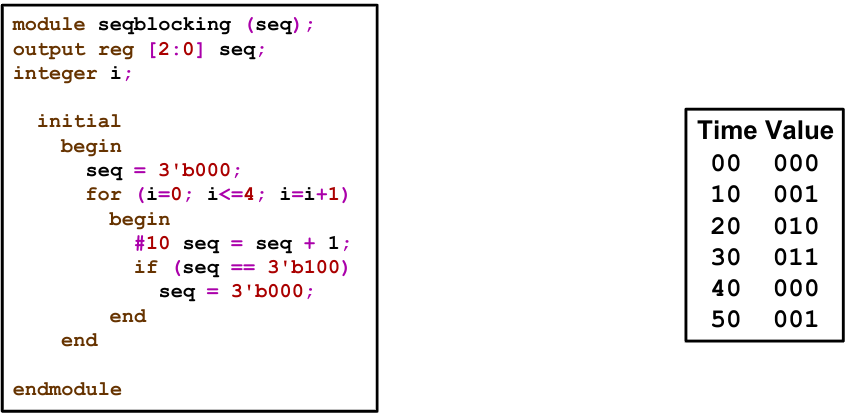
\includegraphics[width=0.95\textwidth]{img/07_block.png}
\end{figure}
\end{frame}
\note{
\scriptsize{
The simulator executes a blocking assignment by evaluating the right-side expression, retaining its value, and blocking further execution of the block until it updates the left-side variable. If the assignment includes an intra-assignment timing control, then the simulator updates the variable after timing control expires, and then continues block execution. If the assignment does not include intra-assignment timing control, then the simulator updated the variable immediately.
\newline

In this example, the \textit{for} loop increments the \textit{seq} signal every 10 time units. The update occurs before the next statement executes. The next statement tests the new value, and if the new value is 4, immediately resets it to 0. The value 4 has no duration, so does not appear in the sequence of monitored values.


}
}

%%%%%%%%%%%%%%%%%%%%%%%%%%%%%%%%%%%%%%%%%%%%%%%%%%%%%%%%%%%%
\begin{frame}
\frametitle{Blocking Assignments in Sequential Procedures}

\end{frame}

%%%%%%%%%%%%%%%%%%%%%%%%%%%%%%%%%%%%%%%%%%%%%%%%%%%%%%%%%%%%
\begin{frame}
\frametitle{Module}

\end{frame}

%%%%%%%%%%%%%%%%%%%%%%%%%%%%%%%%%%%%%%%%%%%%%%%%%%%%%%%%%%%%
\begin{frame}
\frametitle{Module}

\end{frame}

%%%%%%%%%%%%%%%%%%%%%%%%%%%%%%%%%%%%%%%%%%%%%%%%%%%%%%%%%%%%
\begin{frame}
\frametitle{Module}

\end{frame}

%%%%%%%%%%%%%%%%%%%%%%%%%%%%%%%%%%%%%%%%%%%%%%%%%%%%%%%%%%%%
\begin{frame}
\frametitle{Module}

\end{frame}

%%%%%%%%%%%%%%%%%%%%%%%%%%%%%%%%%%%%%%%%%%%%%%%%%%%%%%%%%%%%
\begin{frame}
\frametitle{Module}

\end{frame}

%%%%%%%%%%%%%%%%%%%%%%%%%%%%%%%%%%%%%%%%%%%%%%%%%%%%%%%%%%%%
\begin{frame}
\frametitle{Module}

\end{frame}

%%%%%%%%%%%%%%%%%%%%%%%%%%%%%%%%%%%%%%%%%%%%%%%%%%%%%%%%%%%%
\begin{frame}
\frametitle{Module}

\end{frame}

%%%%%%%%%%%%%%%%%%%%%%%%%%%%%%%%%%%%%%%%%%%%%%%%%%%%%%%%%%%%
\begin{frame}
\frametitle{Module}

\end{frame}

%%%%%%%%%%%%%%%%%%%%%%%%%%%%%%%%%%%%%%%%%%%%%%%%%%%%%%%%%%%%
\begin{frame}
\frametitle{Module}

\end{frame}

%%%%%%%%%%%%%%%%%%%%%%%%%%%%%%%%%%%%%%%%%%%%%%%%%%%%%%%%%%%%
\begin{frame}
\frametitle{Module}

\end{frame}


\end{document}
